\chapter*{Problemas}
\addcontentsline{toc}{chapter}{Problemas}
\markboth{Problemas}{Problemas}
 \paragraph{P1}  
 
 \problembreak
 
 \paragraph{P2} Fuerza bruta
 
 \problembreak
 
 \paragraph{P3} Planetas: 
 
 
 \omegalink{planetas} 
 
  \problembreak
  
 \paragraph{P4} El COMI diseñó unos mapas futuristas. Los mapas futuristas son como los mapas de ahora, pero están impresos en una superficie transparente. Ellos tienen un archivo de varios mapas de la galaxia. Sebastian y Héctor se dieron cuenta de que existen varios mapas repetidos, por lo que desean eliminar cualquier repetición. Para esto, Sebastian toma un mapa, Héctor toma otro y ambos comparan los mapas para determinar si son iguales. Sin embargo, Héctor estaba distraído y algunos mapas se los pasaba en una posición diferente a la original. Ahora necesitan tu ayuda para comparar los dos mapas y saber si son iguales.
 
 Un mapa está representado por una matriz cuadrada de \verb|X|s y \verb|O|s. Dos mapas son iguales si ambos tienen el mismo carácter en la misma coordenada, para todas las coordenadas.
 
 Para validar que dos mapas son iguales, puedes aplicar cualquiera de las siguientes acciones cero o más veces sobre un mapa que quieras comparar con otro:
 \begin{plimits}
 	\item Rotarlo 90º.
 	\item Rotarlo 180º.
 	\item Rotarlo 270º.
 	\item Invertirlo horizontalmente.
 	\item Invertirlo verticalmente.
 \end{plimits}
 \begin{center}
 	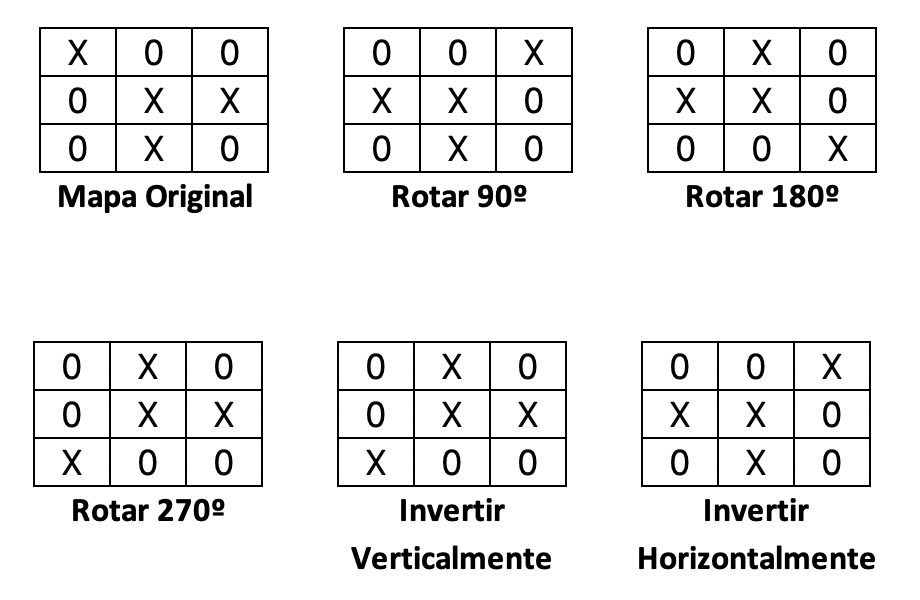
\includegraphics[scale=0.55]{mapasOMI2020}
 \end{center}
 
 \subsubsection*{Problema}
 Se te mostrará dos mapas y debes ayudarles a decir si son iguales o diferentes. Si son iguales, deberás escribir \verb|IGUALES|. Si son diferentes, deberás escribir \verb|DIFERENTES|.
 
 \subsubsection*{Entrada}
 En la primera línea \(N\), la longitud del lado de cada mapa. En las siguientes \(N\) líneas una cadena de \(N\) caracteres \verb|O| ó \verb|X| que representan el primer mapa. En las siguientes \(N\) líneas una cadena de \(N\) caracteres \verb|O| ó \verb|X| que representan el segundo mapa.
\subsubsection*{Salida}
Debes escribir \verb|IGUALES| si los mapas son iguales después de hacer todas las transformaciones necesarias o \verb|DIFERENTES| en caso contrario.

\subsubsection*{Ejemplo}
\begin{casebox3}
	\ecase{
		4\\
		XOOO\\
		XXOO\\
		OOOO\\
		XXXX\\
		XOOO\\
		XOOO\\
		XOXO\\
		XOXX
	}{IGUALES}{Si el segundo mapa lo giras 90º y además\\ lo inviertes verticalmente, obtienes \\la misma distribución que el primer mapa.}
	\ecase{
		2\\
		XX\\
		OO\\
		XO\\
		OX
	}{DIFERENTES}
	{No hay manera de transformar el segundo \\mapa para que se vea tal como el primero.}
	\ecase{
		4\\
		XOOO\\
		XXOO\\
		OOOO\\
		XXXX\\
		XOOO\\
		XXOO\\
		OOOO\\
		XXXX
	}{IGUALES}{
		En este caso los mapas ya son iguales,\\ sin necesidad de aplicar ninguna operación.		
	}
\end{casebox3}

\subsubsection*{Límites}
\(1 \leq N \leq 500\)
\subsubsection*{Subtareas}
\begin{plimits}
	\item (25 puntos)
	\begin{plimits}
		\item \(1\leq N \leq 10\)
		\item Se asegura que, en caso de que los mapas sean iguales, no es necesario aplicar ninguna acción.
	\end{plimits}
	\item (25 puntos)
	\begin{plimits}
		\item \(1\leq N \leq 50\)
		\item Se asegura que, en caso de que los mapas sean iguales, no es necesario aplicar ninguna rotación.
	\end{plimits}
	\item (25 puntos)
	\begin{plimits}
		\item \(1\leq N \leq 50\)
		\item Se asegura que, en caso de que los mapas sean iguales, no es necesario aplicar ninguna inversión vertical o inversión horizontal.
	\end{plimits}
	\item (25 puntos)
	\begin{plimits}
		\item \(1\leq N \leq 500\)
		\item Cualquier acción podría ser necesaria para validar que los mapas son iguales.
	\end{plimits}
\end{plimits}
 Fuente: \textbf{OMI 2020}
 
 \omegalink{OMI-2020-Mapas}
 
 
 \problembreak
 
 \paragraph{P5} DUMMY TODO
 
 
 \problembreak
 
 \paragraph{P6} DUMMY TODO


\problembreak
 
 \paragraph{P7} La siguiente lección en preparatoria requiere que dos temas sean discutidos. El i-ésimo tema es interesante por \(a_i\) unidades para el profesor y \(b_i\) unidades para los estudiantes.
 
 Un par te temas \(i\) y \(j\) (\(i<j\)) es llamado \textbf{bueno} si \(a_i+a_j > b_i+b_j\) (es decir, es más interesante para el profesor).
 
 Tu tarea es encontrar el número de parejas de temas \textbf{buenas}.
 \subsubsection*{Entrada}
 Un entero \(n\), la cantidad de temas.
 
 La segunda línea tiene \(n\) enteros: \(a_1,a_2,\ldots, a_n\), donde \(a_i\) es cuan interesante es el tema \(i\) para el profesor.
 
 La tercera línea tiene \(n\) enteros: \(b_1,b_2,\ldots, b_n\), donde \(b_i\) es cuan interesante es el tema \(i\) para los estudiantes.
 
 \subsubsection*{Salida}
 Un entero, la cantidad de parejas buenas.
 
 \subsubsection*{Ejemplo}
 \begin{casebox2}
 	\scase{
	 	5\\
	 	4 8 2 6 2\\
	 	4 5 4 1 3
 }{7}
	\scase{
		4\\
		1 3 2 4\\
		1 3 2 4
	}{0}
 \end{casebox2}

\subsubsection*{Límites}
\begin{plimits}
	\item \(2\leq N\leq 2\cdot 10^5\)
	\item \(1\leq a_i, b_i\leq  10^9\)
\end{plimits}
 \codeforces
 
 \codeforceslink{1324}{D} 
 

\problembreak

 \paragraph{P8} La leyenda dice que el tesoro de Moctezuma está enterrado en el Centro Histórico de la Ciudad de México. El Centro Histórico está representado como una cuadrícula de \(n\) filas y \(m\) columnas. Gracias a la tecnología de la nueva app iFind puedes desenterrarlo por fin.
 
 iFind es una app donde especificas una casilla \((i,j)\) de la cuadrícula y la app responde cuántos tesoros hay enterrados en el área del rectángulo que abarca de la fila \(1\) a la fila \(i\) y de la columna \(1\) a la columna \(j\).
 
 Una vez que sabes la casilla exacta donde hay un tesoro debes cavar en esa posición para desenterrarlo.
 
 Se asegura que cada casilla solo puede tener  o  tesoro y que no hay más de  tesoro en cada columna.
 
 \subsubsection*{Problema}
 Escribe un programa que dados \(n\) y \(m\), el alto y ancho de la cuadrícula y \(k\), el número total de tesoros enterrados, desentierre los \(k\) tesoros usando la menor cantidad posible de preguntas a la app.
 
 \subsubsection*{Interacción}
 No necesitas leer o escribir\footnote{Este es un problema interactivo, si no conoces como trabajar con estos, ve la página: \pageref{interactivos}}, debes implementar en tu código la función \verb|BuscaTesoros| y mandar llamar las funciones del evaluador \verb|Preguntar| y \verb|Cavar| para completar tu tarea.
 
 Internamente el evaluador llevará el registro de cuántos tesoros quedan. Tu programa no necesitará imprimir ni devolver nada: solo asegurarse de que hayas desenterrado los  tesoros usando la función Cavar.
 
\subsubsection*{Implementación}
\verb|void BuscaTesoros(int n, int m, int k);|

\textbf{Descripción:} El evaluador buscará en tu código esta función y la llamará con los parámetros \verb|n|, \verb|m| y \verb|k|. Tu implementación deberá utilizar las funciones \verb|Preguntar| y \verb|Cavar| para desenterrar todos los tesoros. En cada caso de prueba solo se llamará a esta función una vez.

\textbf{Parámetos}
\vspace{-\baselineskip}
\begin{plimits}
	\item \verb|n|: Filas de la cuadrícula.
	\item \verb|m|: Columnas de la cuadrícula.
	\item \verb|k|:  El número de tesoros enterrados.
\end{plimits}

TODO COMPLETAR

Fuente: \textbf{OMI 2018}
 
\omegalink{OMI2018-Tesoro}

\problembreak